\chapter{Extension to Maximum Matching}
\label{chap:maximum_matching}

This chapter shows how to extend the perfect matching algorithms to solve the maximum matching problem.

\section{Maximum Matching algorithm}

The extension to maximum matching is based on the following theorem by Lovasz.
\begin{theorem}[\citet{plummer1986matching}]
\label{thm:rank_matching}
    Let \(G\) be a graph and let \(T\) be the Tutte Matrix of \(G\).
    Then, \(\rank(T_G) = 2\nu(G)\).
\end{theorem}

\begin{proof}
  See \citet[p.~560]{Rabin1989}.
\end{proof}

According to \cref{thm:rank_matching}, the number of unmatched vertices can be directly computed as:
\[
    |V(G)| - \rank(T).
\]
To address these unmatched vertices, we can construct an augmented graph by introducing new vertices connected to all existing vertices. 
Specifically, for each unmatched vertex in the original graph, we add a new vertex with connections to every vertex in the original graph. 
This transformation ensures that every previously unmatched vertex now has an adjacent vertex, thus ensuring the existence of a perfect matching.

\newpage
\begin{programruledcaption}{Maximum Matching algorithm}
    \begin{lstlisting}[
      language={pseudocode},
      style=pseudocode,
      style=wider,
      functions={PerfectMatching, TutteMatrix, Rank},
      specialidentifiers={},
    ]
        function MaximumMatching(G)
            $T$ := TutteMatrix(G) // Tutte matrix of \(G\) with random values.
            $G'$ := $G$
            for i := 0; i < |V(G)| - rank(G); i := i + 1 
                $v$ := new vertex
                $V(G')$ := $V(G') \cup \{v\}$
                for $u \in V(G)$ do 
                    $E(G')$ := $E(G') \cup \{uv\}$
            $M'$ := PerfectMatching($G'$)
            $M$ := $\emptyset$
            for $uv \in M'$ do 
                if $u \in E(G)$ and $v \in V(G)$ then // If this edge exists in the original graph.
                    $M$ := $M \cup \{uv\}$
            return M
    \end{lstlisting}
\end{programruledcaption}

\subsubsection{Time complexity}
\noindent
Let \(t(G)\) be the total running time of \(\SC{MaximumMatching}(G)\) and \(f(G)\) be the running time of \(\SC{PerfectMatching}(G)\). Then, we have
\begin{itemize}
\item \textbf{Augmented Graph creation (Lines 4 to 10)}:
The algorithm identifies unmatched vertices and adds corresponding new vertices. 
Since there are at most \(n\) unmatched vertices and each new vertex connects to \(n\) vertices, this phase requires \(O(n^2)\) time;

\item \textbf{Perfect Matching in the augmented graph (Line 11)}: 
The augmented graph has at most \(2n\) vertices. 
By \cref{alg:harvey_complexity}, this step has a time complexity  \(f(G') = O((2n)^\omega) = O(2^\omega n^\omega) = O(n^\omega)\);

\item \textbf{Maximum Matching recovery (Lines 13 to 17)}: 
Checking whether a vertex belongs to the original graph can be implemented in \(O(1)\) time by using integer indexing. 
The overall complexity for this verification across all vertices is \(O(n)\).
\end{itemize}
Combining these steps, the total time complexity is:
\[
t(G) = O(n^2) + f(G') + O(n^2) = O(n^2) + O(n^\omega) + O(n^2) = O(n^\omega). \numberthis \label{alg:maximum_matching_complexity}
\]

\section{Analysis}
\label{Maximum:analysis}

\subsection{Methology}

\subsection{Results}

\begin{figure}[H]
  \centering
  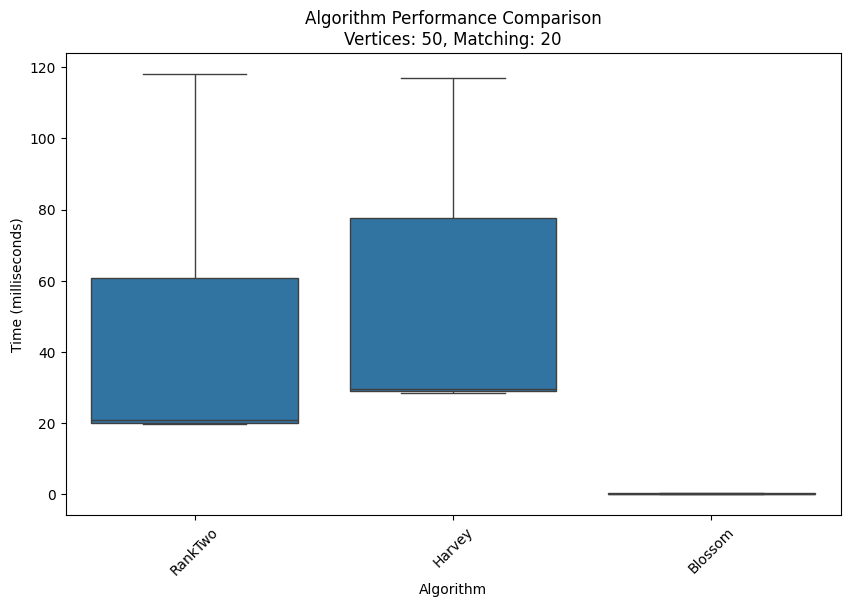
\includegraphics[width=12cm]{boxplot_v50_m20.png}
  \caption{Maximum Matching benchmark with 50 vertices and matching number 20.}
  \label{fig:v50m20}
\end{figure}
\begin{figure}[H]
  \centering
  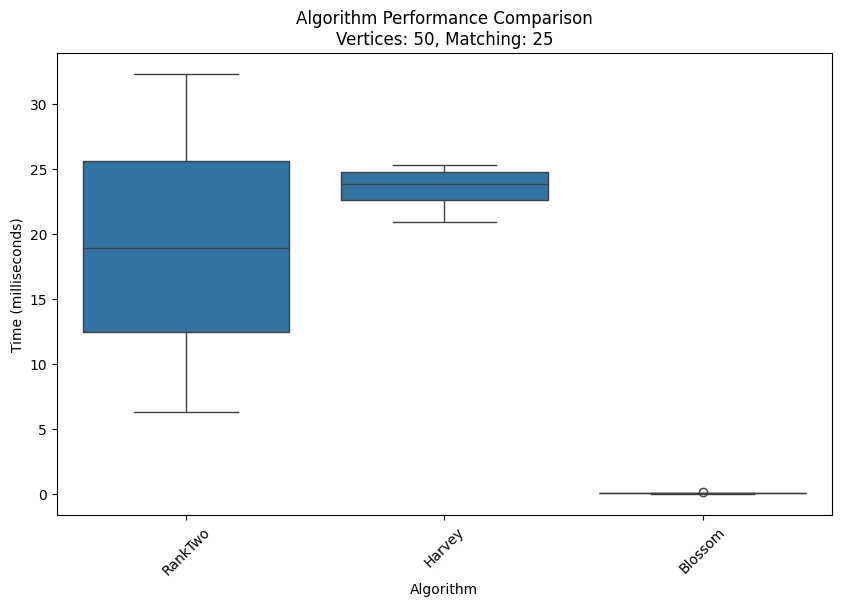
\includegraphics[width=12cm]{boxplot_v50_m25.png}
  \caption{Maximum Matching benchmark with 50 vertices and matching number 25.}
  \label{fig:v50m25}
\end{figure}
\begin{figure}[H]
  \centering
  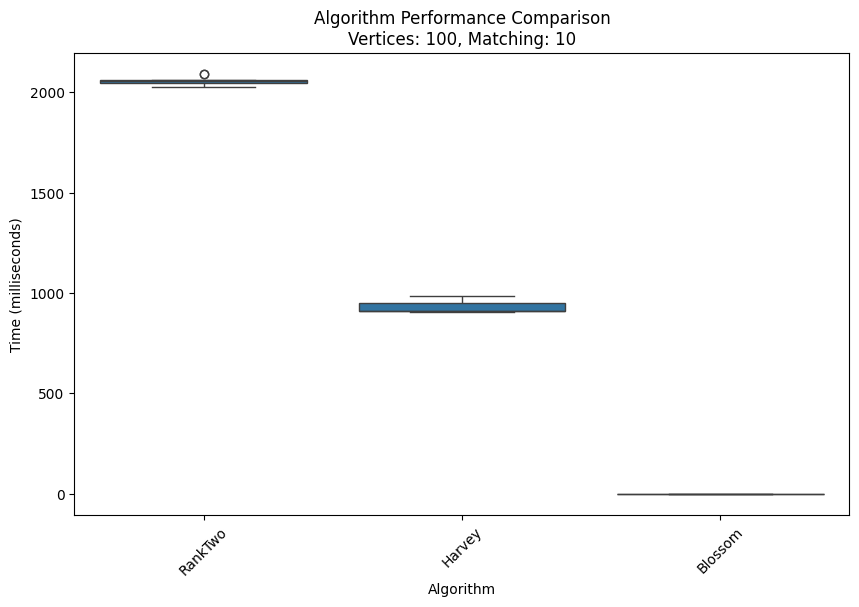
\includegraphics[width=12cm]{boxplot_v100_m10.png}
  \caption{Maximum Matching benchmark with 100 vertices and matching number 10.}
  \label{fig:v100m10}
\end{figure}
\begin{figure}[H]
  \centering
  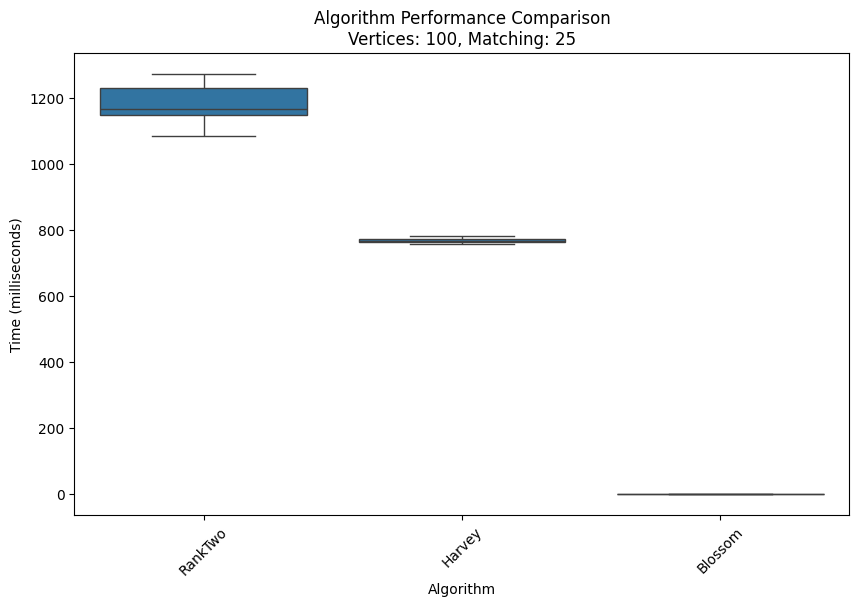
\includegraphics[width=12cm]{boxplot_v100_m25.png}
  \caption{Maximum Matching benchmark with 100 vertices and matching number 25.}
  \label{fig:v100m20}
\end{figure}
\begin{figure}[H]
  \centering
  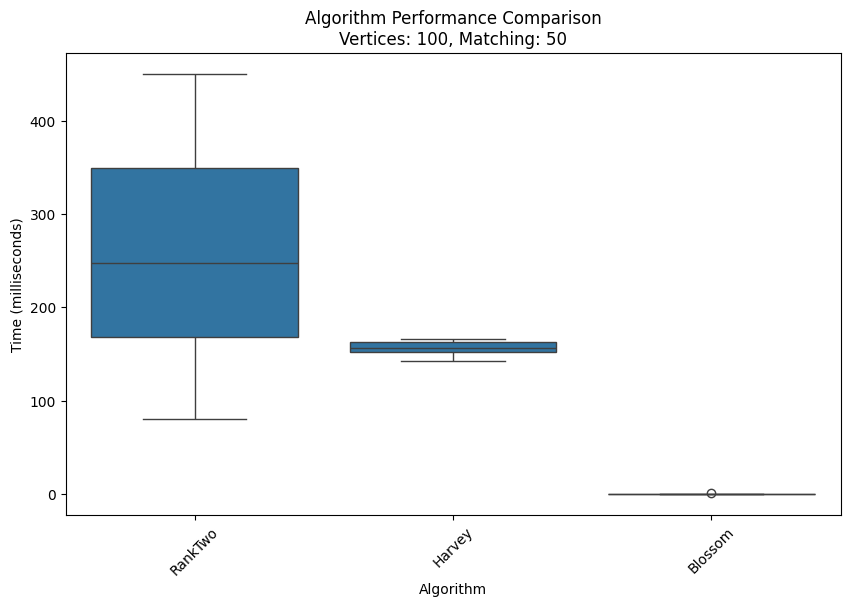
\includegraphics[width=12cm]{boxplot_v100_m50.png}
  \caption{Maximum Matching benchmark with 100 vertices and matching number 50.}
  \label{fig:v100m50}
\end{figure}
% \begin{figure}[H]
%   \centering
%   \includegraphics[width=12cm]{boxplot_vX_mY.png}
%   \caption{Maximum Matching benchmark with X vertices and matching number Y.}
%   \label{fig:vXmY}
% \end{figure}
